\documentclass[12pt,a4paper]{article}
\usepackage[utf8]{inputenc}
\usepackage[german]{babel}
\usepackage[T1]{fontenc}
\usepackage{amsmath}
\usepackage{amsfonts}
\usepackage{amssymb}
\usepackage{graphicx}
\usepackage[left=2.5cm,right=2.5cm,top=2cm,bottom=2cm]{geometry}
\usepackage{float}
\author{Gruppe C14 \\ Julián Häck, Martin Koytek, Lars Wenning, Erik Zimmermann}
\begin{document}
\section{Bestimmung der Erdbeschleunigung mit dem Pendel}
\subsection{Versuchsbeschreibung}
%Kurze Darstellung der physikalischen Grundlagen und Ziele der Versuche, %die zum Verständnis
%des Versuches/Protokolls benötigt werden. (max. 1 Seite)
Wir betrachten zunächst ein mathematisches Pendel($J=m_Tl^2$) welches wir später durch die Verschiebung des Pendelkörpers ergänzen um das physikalische Pendel betrachten zu können.
Die Bewegungsgleichung zum mathematischen Pendel nach der Kleinwinkelnäherung lautet:
\begin{equation}
J \cdot \ddot{\phi} = -m_s \cdot g \cdot l \cdot \phi 
\end{equation}
Mit $m_T=m_S$ und Lösen der Differential-Gleichung ergibt sich die allgemeine Lösung einer harmonischen Schwingung:
\begin{equation}
\phi(t)=A\cdot cos(\omega t) + B \cdot sin(\omega t)
\end{equation}
mit 
\begin{equation}
\omega=\sqrt{\frac{g}{l}}
\end{equation}
Wir bestimmen zunächst die Frequenz der Pendelstange ohne Gewicht. Dann bringen das Gewicht an verschieben es auf der Stange bis die neue Frequenz mit der alten übereinstimmt. Dadurch erreichen wir, dass wir das gesamte Pendel als homogenen Zylinder mit Radius $r_p$, der im Abstand $l_p$ um den Aufhängepunkt schwingt annehmen können. 
\begin{equation}
J_p=\frac{1}{2}m_p r_p^2+m_p l_p^2
\end{equation}
Mit
\begin{equation}
\omega^2=\frac{D}{J}=\frac{m_p \cdot g \cdot l_p}{\frac{1}{2}m_p r_p^2+m_pl_p^2}
\end{equation}
ergibt sich:
\begin{equation}
g=\omega^2 l_p (1+\frac{r_p^2}{2 l_p^2}) 
\label{g}
\end{equation} 
\newpage
\subsection{Versuchsaufbau und Durchführung}
%Genaue Beschreibung der verwendeten Aufbauten unter Verwendung von Skizzen oder Photos
%Beschreibung der Messwerterfassungseinstellungen (eingestellte Messzeiten, Messbedingungen,
%Trigger, Anzahl der Messungen) und der Durchführung der Versuche. (max. 1 Seite)
\begin{figure}[H]
\centering
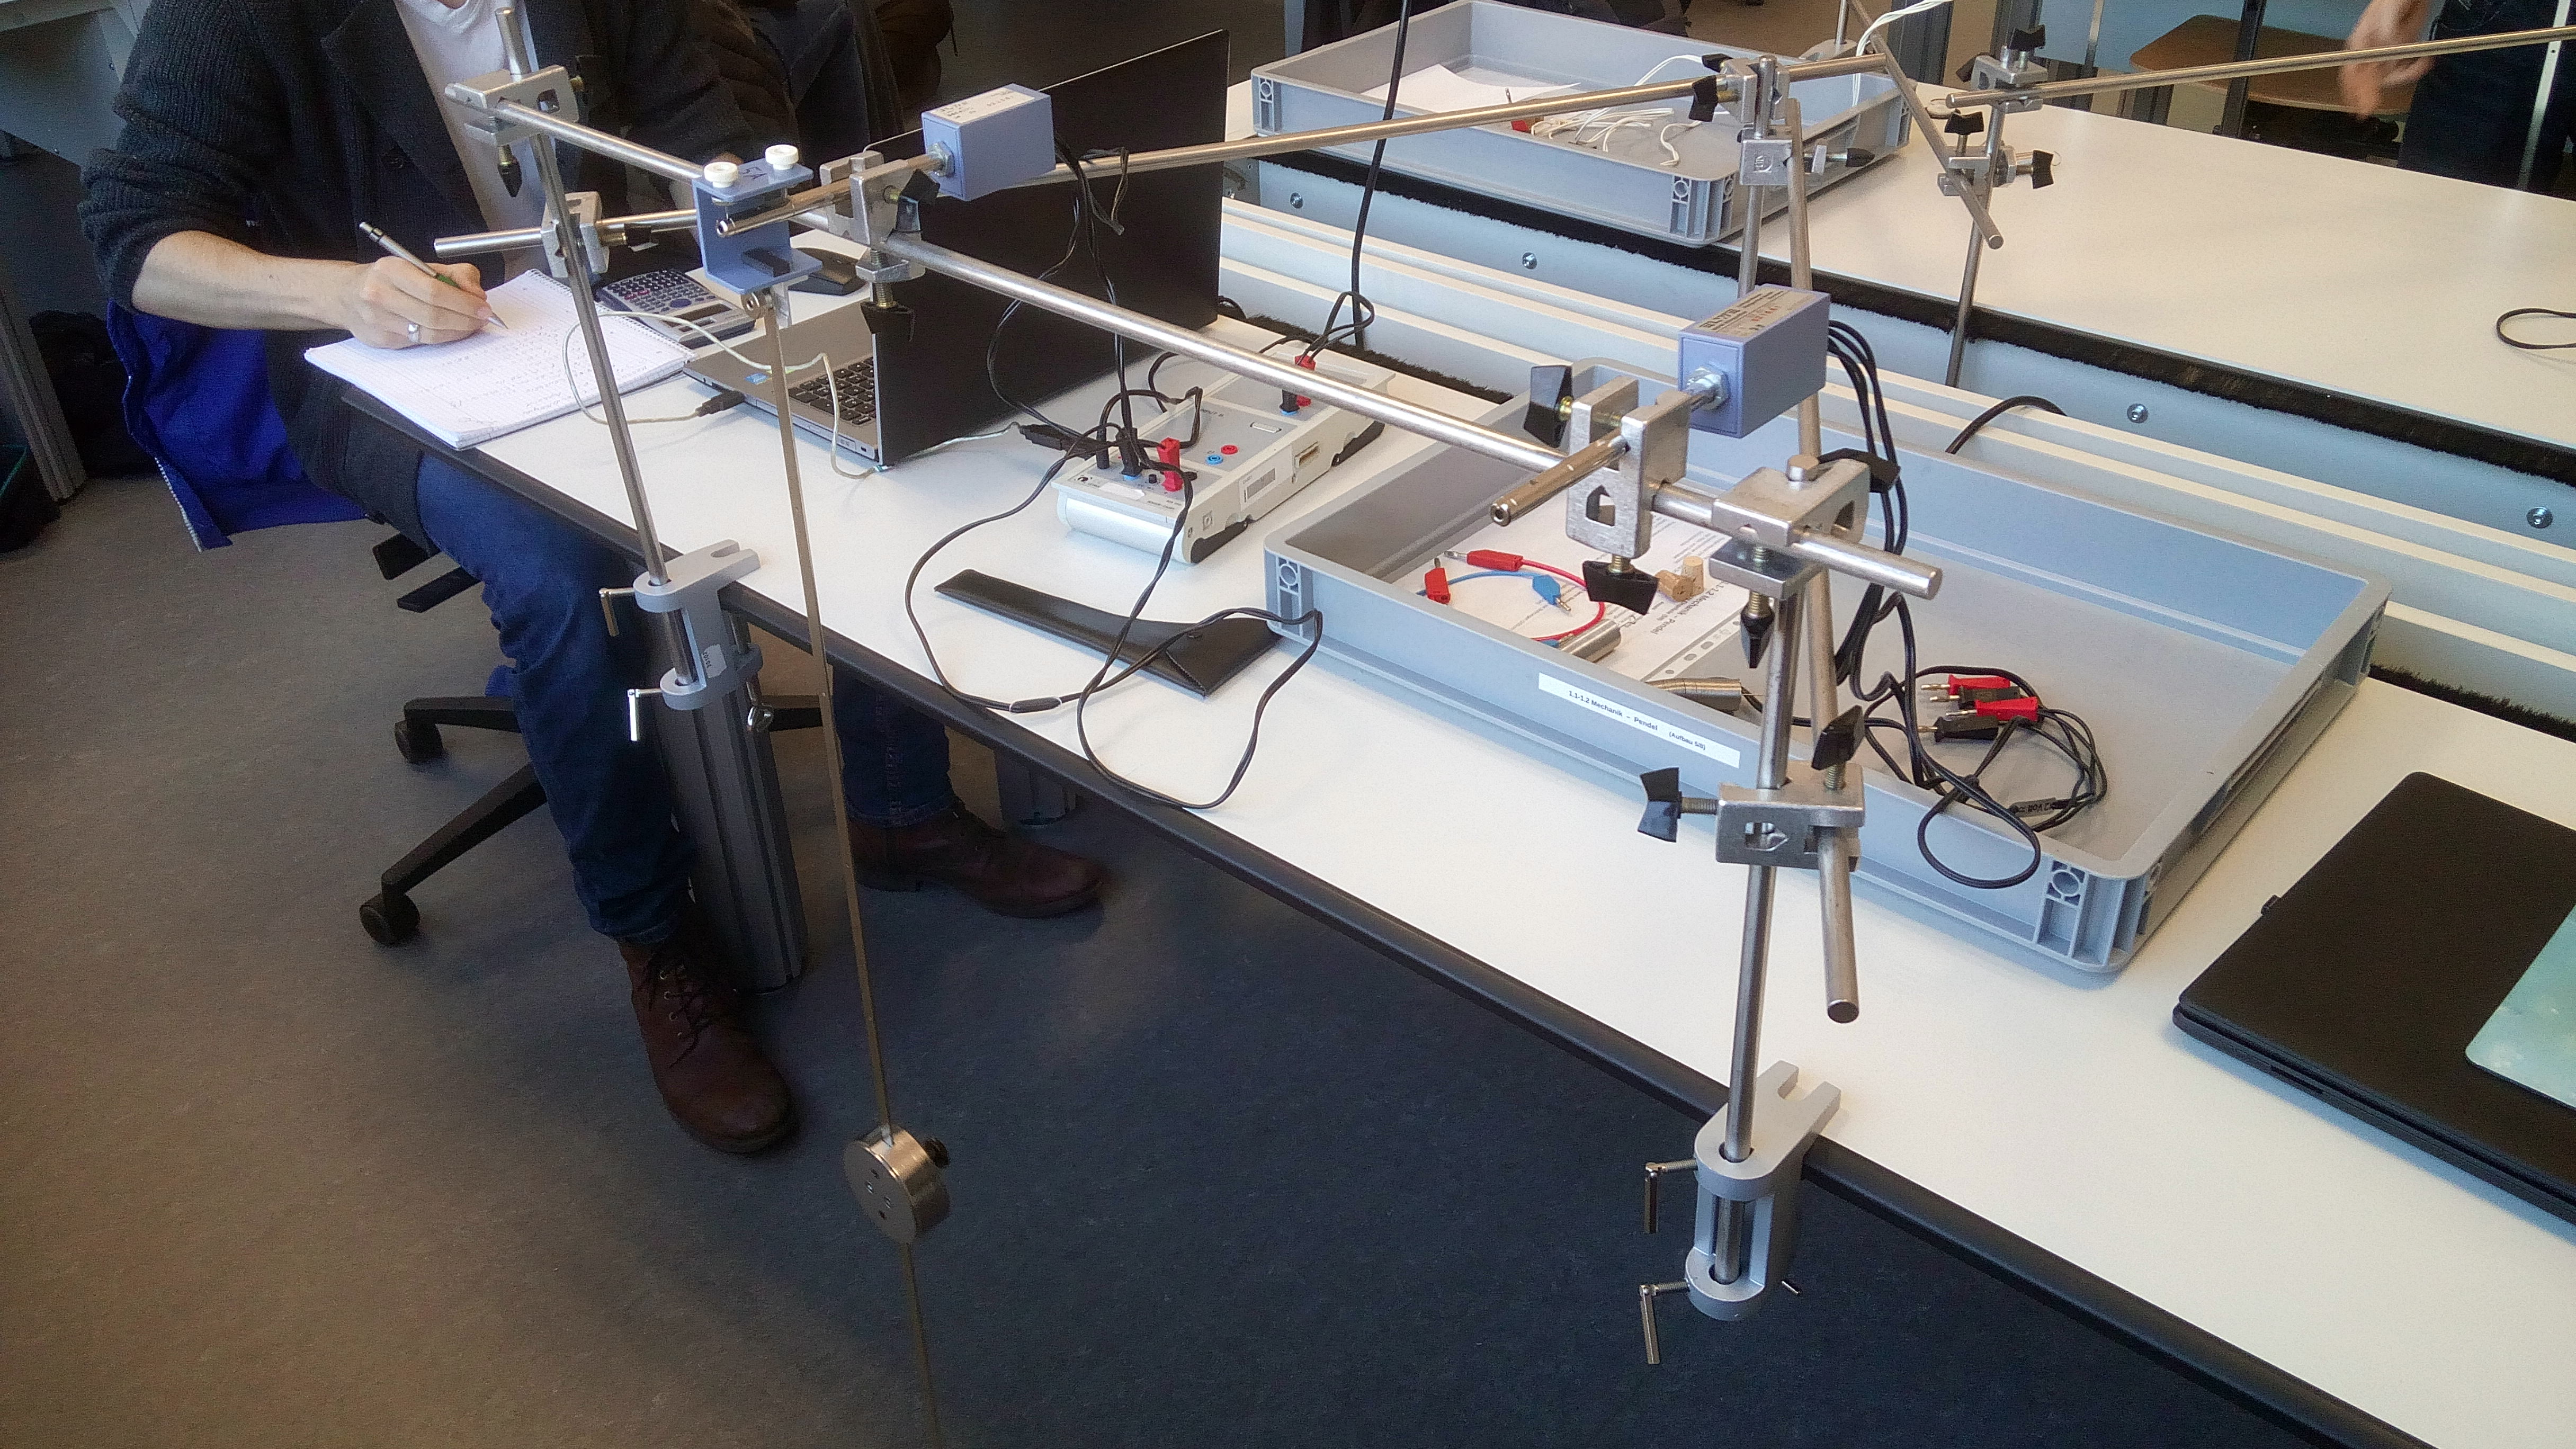
\includegraphics[scale=0.1]{Bilder/Einzelpendel.jpg}
\caption{Versuchsaufbau mit Pendelkörper}
\end{figure}
Unser Versuchsaufbau besteht aus einem Dreibein um die Stabilität zu erhöhen, an dem dann der Winkelabnehmer befestigt wurde. \newline
In die Nut des Winkelabnehmers wurde dann die Aufhängung des Pendels aufgelegt.
Nun wurde zunächst die Pendelstange ohne Pendelkörper in Schwingung versetzt, die Hallspannung des Winkelabnehmers aufgezeichnet und die Frequenz per Fast-Fourier-Transformation (FFT) bestimmt. \newline
Anschließend wurde der Pendelkörper angebracht, das Pendel erneut ausgelenkt und die Schwingung aufgezeichnet. 
Dies wurde wiederholt bis die Frequenz mit der der Pendelstange ohne Pendelkörper übereinstimmte.
Dieser Aufbau wurde nun vier mal in Schwingung versetzt und die Hallspannungen aufgezeichnet.
Zum Schluss wurde dann die Länge des Pendels, der Abstand des Pendelkörpers zum Aufhängepunkt und der Radius des Pendelkörpers gemessen.
\newline
Später haben wir bei der Auswertung alle Frequenzen neu über Ablesen der Nulldurchgänge bestimmt und damit aus Gleichung \ref{g} die Erdbeschleunigung bestimmt.
\subsubsection{Messwerterfassungseinstellungen}
\begin{center}
\begin{tabular}{c|c}
Messbereich & -1V..1V \\ 
\hline
Messintervall & 10ms \\ 
\hline
Messpunkte & 16000 \\ 
\hline
Messzeit & 160s \\ 
\end{tabular} 
\end{center}
\newpage
\subsubsection{Geräte}
Je Gruppe:
\begin{itemize}
\item 2 Hallsonden
\item 1 Laptop
\item 1 Sensor-Cassy
\item 1 Pendelstange mit Aufhängung
\item 1 Gewicht
\item Stativzubehör
\end{itemize}
\subsection{Versuchsauswertung}

\subsubsection{Rohdaten}
\begin{center}
\begin{tabular}{c|c|c}
 & Gruppe 1 & Gruppe 2 \\ 
\hline
Masse & 1.0207kg & 1.0217kg \\ 
$\sigma_{Masse}$ & 0.001kg & 0.001kg \\ 
Durchmesser des Gewichts & 0.08m & 0.084m \\ 
$\Rightarrow$ Radius & 0.04m & 0.042m \\ 
$\sigma_{Schieblehre}$ & 0.0005m & 0.0005m \\ 
$l_p$ & 0.6788m & 0.689m \\ 
$\sigma_{l_p}$ & 0.01m & 0.01m \\ 
Frequenz ohne Gewicht [FFT] & 0.6039Hz & 0.6030Hz \\ 
bsp. Frequenz mit Gewicht [FFT] & 0.6032Hz & 0.6011Hz \\ 
\end{tabular} 
\end{center}
$\sigma_{Masse}$: aus Angabe der Waage.\\
$\sigma_{Schieblehre}$: aus Angabe der Schieblehre. \\
$\sigma_{l_p}$: Durch Durchhängen und Verschieben des Maßbands, Mehrfachmessung der Einzellängen (Radius, Aufhängung, Stange selbst) abgeschätzt.\\
Abweichung Frequenz ohne Gewicht und mit Gewicht:
\begin{equation}
1-\frac{f_o}{f_m}
\end{equation}
\begin{figure}[H]\centering
\begin{tabular}{c|c|c}
 & Gruppe 1 & Gruppe 2 \\ 
\hline
$\Delta f$ & $-1.160\cdot 10^{-3}$ & $-3.161\cdot 10^{-3}$ \\ 
\end{tabular} 
\caption{Abweichungen der Frequenzen}
\label{Abweichungen der Frequenzen}
\end{figure}
\newpage
\subsubsection{Transformation der Rohdaten}
%Transformation der Rohdaten und Modellanpassung. (1 Seite)
Die Frequenzen der  Einzelmessungen mit Pendelkörper wurden folgendermaßen durch Ablesen bestimmt:
\begin{figure}[H]
\caption{Bestimmung von f}
\centering
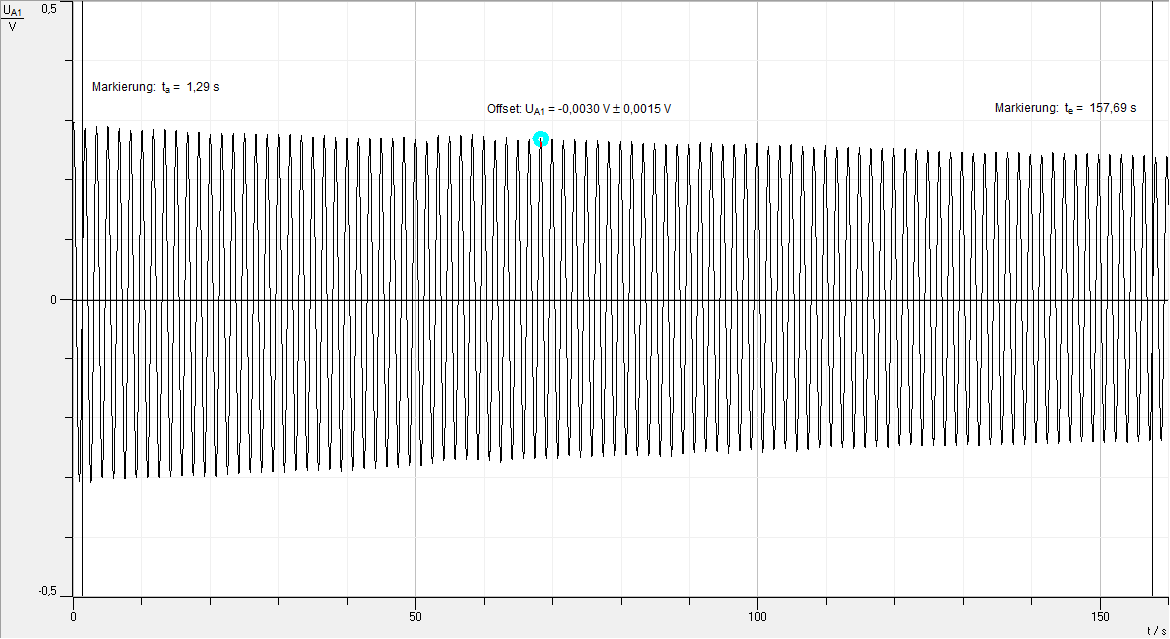
\includegraphics[scale=0.5]{Bilder/Erdbeschleunigung_bestimmungF.png}
\end{figure}
Hier:
\begin{equation}
t_a=1.29s, \hspace{1cm} t_e=157.69s.
\end{equation}
Die Fehler auf die Zeit ergeben sich aus der Auflösung zu:
\begin{equation}
\sigma_t=\frac{0.01}{\sqrt{12}}s
\end{equation}
Um die Nulldurchgänge ordentlich abzulesen, wurde der Mittelwert der Schwingung eingezeichnet. Hier: $U_{Offset} = -0,0030 V$.
Dann wurden die Perioden gezählt. Hier: $n=94$.
Mit Hilfe von:
%w=(2*np.pi*n)/(t_e-t_a)
%sig_w=2*np.pi*np.sqrt(2)*sig_t*n/((t_e-t_a)**2)
\begin{equation}
\omega=\frac{2\pi n}{t_e-t_a}
\end{equation}
und
\begin{equation}
\sigma_{\omega}=\frac{2\cdot \pi \sqrt{2}\cdot n \cdot \sigma_t}{(t_e-t_a)^2}
\end{equation}
wurden jeweils die Kreisfrequenz und deren Fehler bestimmt.
Aus diesen wurde dann durch:
\begin{equation}
g=\omega^2 l_p (1+\frac{r_p^2}{2 l_p^2}) 
\end{equation}
und
\begin{equation}
\sigma_g=\sqrt{(2\omega l_p (1+\frac{r_p^2}{2 l_p^2}))^2 \cdot \sigma_{\omega}^2+(\omega^2 \cdot \frac{r_p}{l_p})^2 \cdot \sigma_r^2+(\omega^2(1-\frac{r_p^2}{2 l_p^2}))^2 \cdot \sigma_l^2} 
\end{equation}
die Erdbeschleunigung und deren Fehler bestimmt.
Daraus ergaben sich folgende Ergebnisse:
\begin{figure}[H]\centering
\begin{tabular}{c|c|c|c|c}
Messung: & 1. & 2. & 3. & 4. \\ 
g: Gruppe 1 & 9.766 & 9.766 & 9.770 & / \\ 
$\sigma_g$: Gruppe 1 & 0.071 & 0.072 & 0.072 & / \\ 
g: Gruppe 2 & 9.838 & 9.839 & 9.842 & 9.845 \\ 
$\sigma_g$: Gruppe 2 & 0.142 & 0.142 & 0.142 & 0.142 \\ 
\end{tabular} 
\newline
\newline
Angaben in $\frac{m}{s^2}$
\end{figure}

Diese Ergebnisse wurden nun gewichtet gemittelt:
\begin{equation}
\bar{g} = \frac{\sum{\frac{g}{(\sigma_g^2}}}{\sum{\frac{1}{\sigma_g^2}}}
\end{equation}
\begin{equation}
\sigma_{\bar{g}} = \sqrt{\frac{1}{\sum{\frac{1}{\sigma_g^2}}}}
\end{equation}
\begin{center}
\begin{tabular}{c|c|c}
 & Gruppe 1 & Gruppe 2 \\ 
\hline 
$\bar{g}$ & 9.767 & 9.841 \\ 
$\sigma_{\bar{g}}$ & 0.041 & 0.071 \\ 
\end{tabular} 
\newline
\newline
Angaben in $\frac{m}{s^2}$
\end{center}


\newpage
\subsubsection{Analyse und Fazit}
\begin{figure}[H]
\caption{Vergleich gewichteter Mittelwert gegen Einzelwerte und theoretischen Wert}
\centering
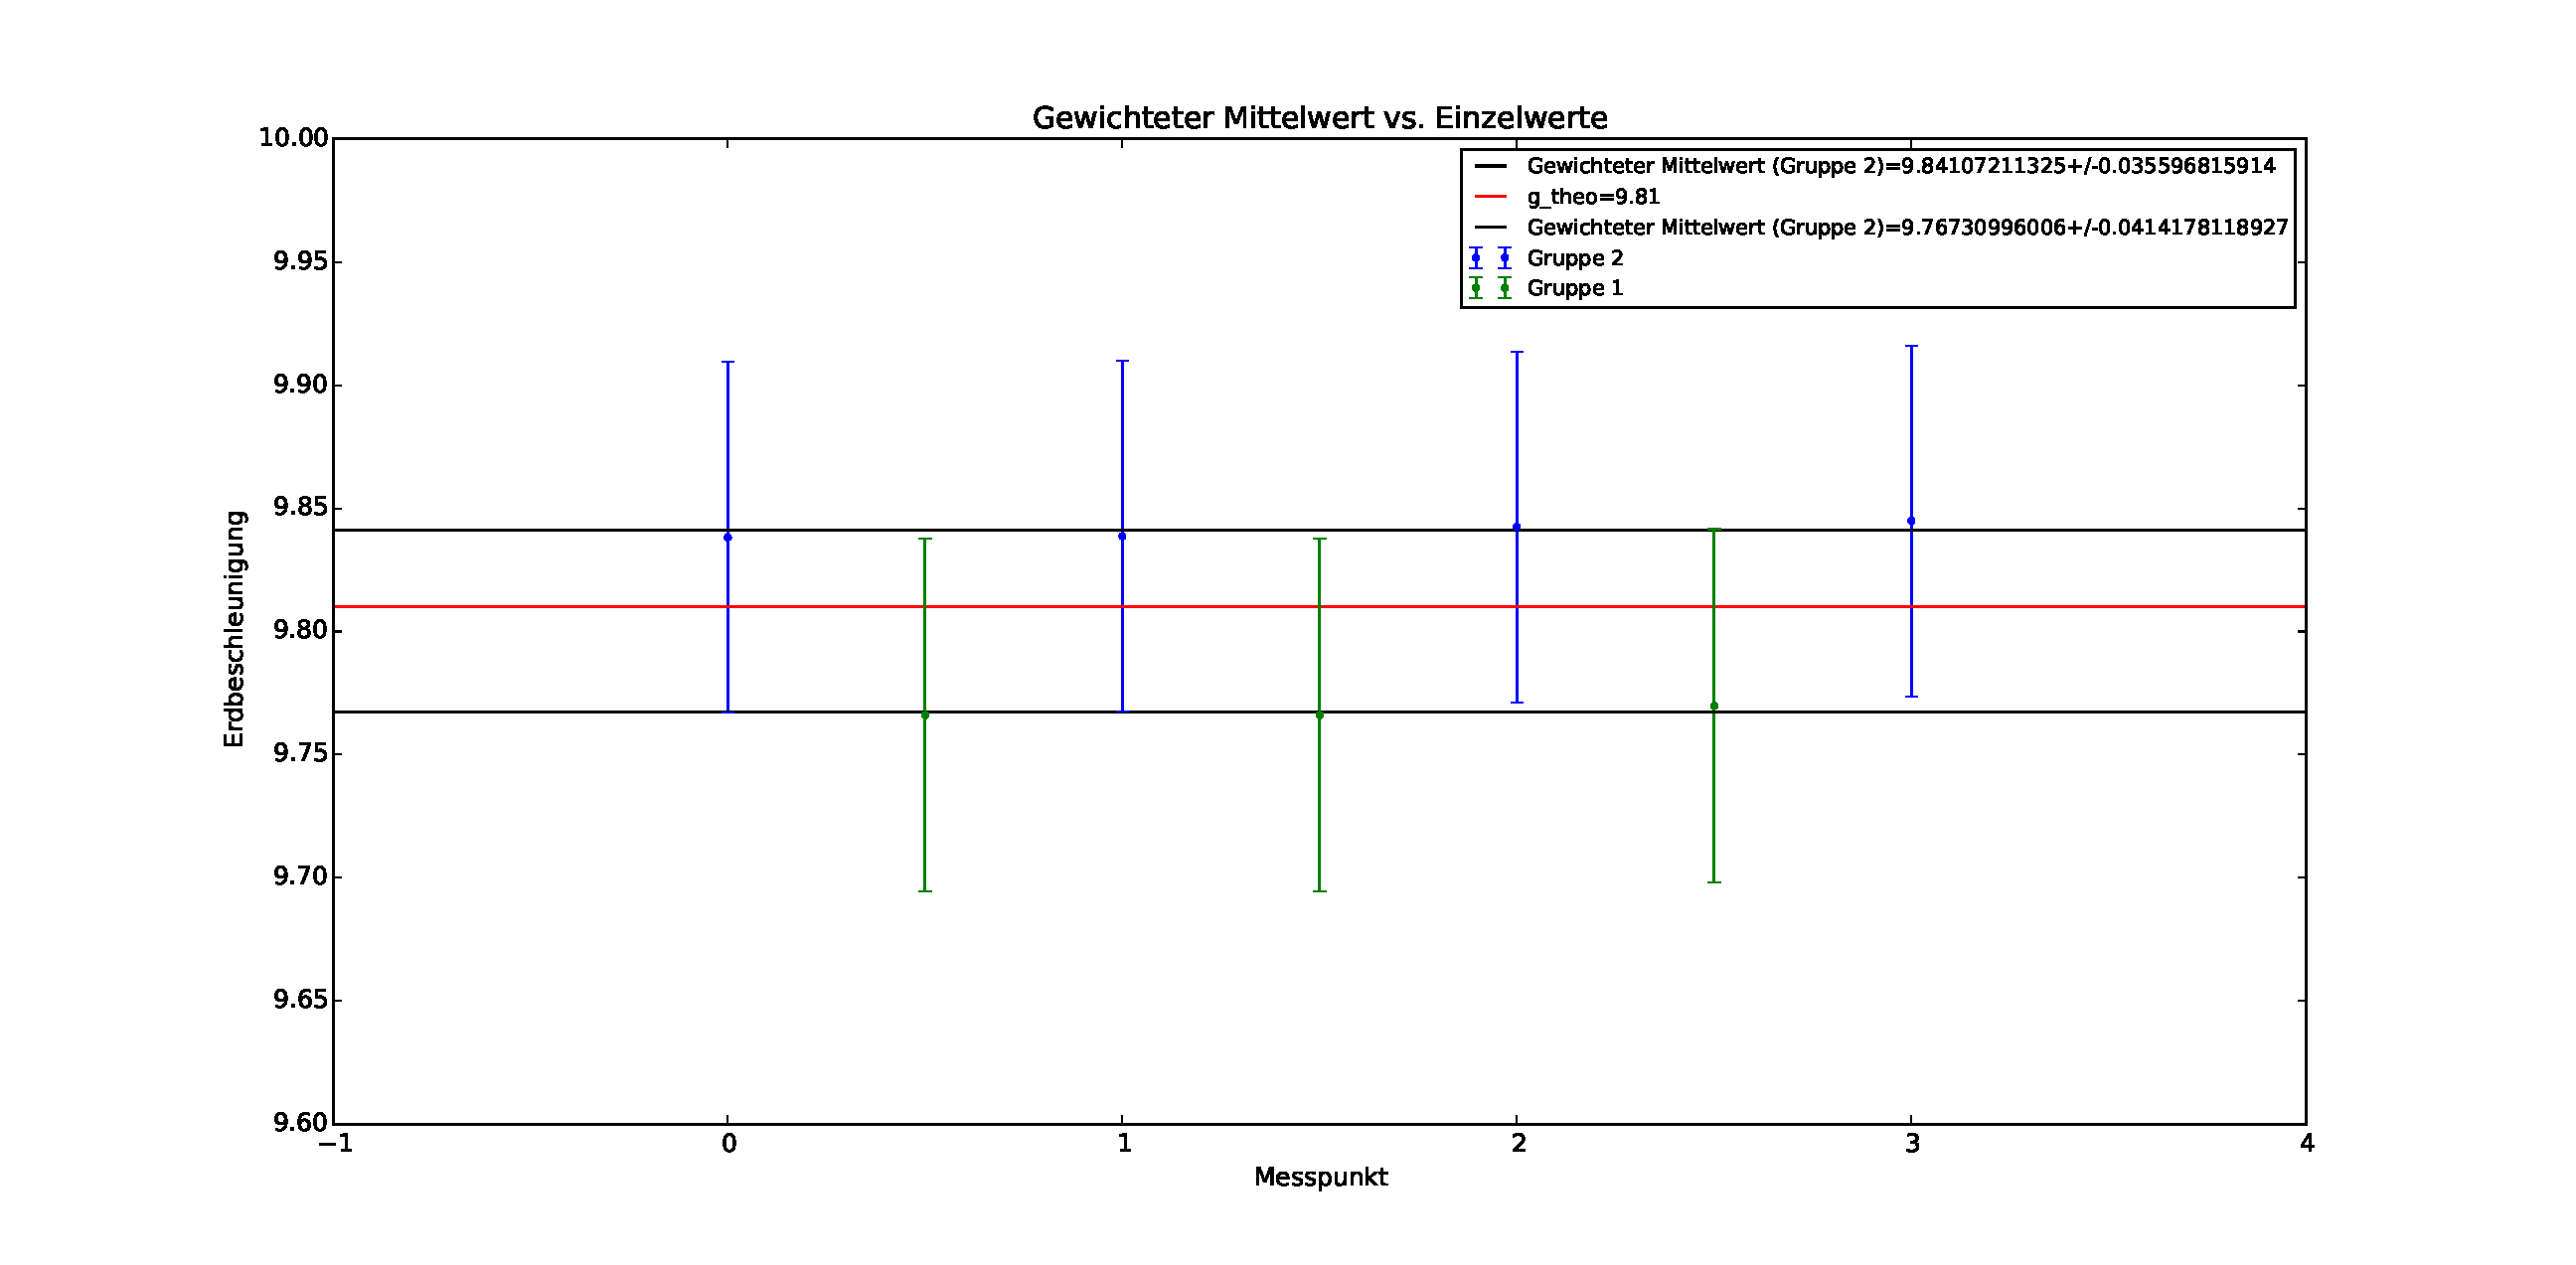
\includegraphics[scale=0.4]{Bilder/Erdbeschleunigung_alle.eps}
\end{figure}
Auf dem Plot sehen wir in grün die Einzelwerte mit Einzelfehler für g der Gruppe 1 mit ihrem gewichteten Mittelwert, darüber ist in blau dasselbe für Gruppe 2 eingezeichnet. In rot sehen wir in der Mitte den theoretischen Wert von $g=9.81$.
\newline
Wie man sieht schneiden alle Fehlerbalken sowohl den gewichteten Mittelwert, als auch den theoretischen Wert von g. Interessant hierbei ist, dass Gruppe 1 stets unterhalb des theoretischen Wertes geblieben ist und Gruppe 2 ausschließlich darüber.
Dies kann man durch die Annahme erklären, die wir weiter oben gemacht haben, nämlich, dass das Pendel mit Pendelkörper, wenn es die gleiche Frequenz wie das Pendel ohne Pendelkörper hat, durch einen Zylinder genähert werden kann. 
Wie in der Tabelle der Rohdaten zu sehen ist sind die Frequenzen des Pendels damit und ohne Gewicht nicht exakt gleich(siehe Abbildung: \ref{Abweichungen der Frequenzen}). Dies wirkt sich auf unsere Näherung aus und erklärt so unsere Abweichung im obenstehenden Plot.\\

\textbf{Fazit}: \newline
Zusammenfassend kann man sagen, dass unsere Ergebnisse sehr zufriedenstellend sind. Sie weichen zwar systematisch vom theoretischen Wert ab, dies lässt sich aber durch die Näherung des homogenen Zylinders erklären.
\end{document}